\documentclass[11pt]{article}
\usepackage[letterpaper,margin=1in]{geometry}
\usepackage{amsmath,amssymb,amsthm}
\usepackage{graphicx}
\usepackage{xcolor}
\usepackage[colorlinks,linkcolor=blue!50!black,citecolor=blue!50!black,
            urlcolor=blue!50!black,pdfencoding=auto]{hyperref}
\newtheorem{theorem}{Theorem}
\providecommand{\tightlist}{\setlength{\itemsep}{0pt}\setlength{\parskip}{0pt}}
\setlength{\emergencystretch}{2em}
\setlength{\parskip}{2pt plus 1pt}
\setlength{\textfloatsep}{17pt plus 3pt minus 4pt}
\setlength{\intextsep}{12pt plus 3pt minus 3pt}
\raggedbottom
\title{Rare Common-Shock Detection from Binary Snapshots\\[3pt]
  \large Minimum cover order and optimal inspection}
\author{}
\date{Research draft for discussion \textbullet{} 9 November 2026}
\hypersetup{pdftitle={Rare Common-Shock Detection from Binary Snapshots}}
\begin{document}
\maketitle
\begin{abstract}
We compare two rates for a global shock in a system with independent subset shocks. Each replicate is inspected once, yielding the full binary status vector at a chosen time. We vary the global rate while compensating the dedicated rates, so the two candidates have identical one-dimensional margins. In fixed dimension, when the minimum cover uses \(r\ge3\) nonglobal labels and its leading reliability coefficient stays bounded away from zero, we derive the exact asymptotic squared Hellinger separation and characterize every first-order optimal inspection time. The asymptotics are uniform even when the difference of the two vanishing rates is arbitrarily small relative to their sum. At \(r=2\), the leading coefficient is one fourth of the maximum of the baseline Fisher curve over the compactified time axis. A fixed-dimensional example exhibits a strict gain at positive time. For two overlapping background shocks in growing dimension, we give two separation rates and an example in which their ratio diverges at matched global and background rates, total block count, and marginal calibration.
\end{abstract}

\section{Introduction}\label{introduction}

Suppose that a replicated system is inspected once after a prescribed exposure. The status of every block is recorded, but the order and timing of individual events are unavailable. A global shock can produce the same all-complete snapshot as several smaller shocks occurring before inspection. Inspecting too early misses the global event. Inspecting too late lets other mechanisms produce the same observation. We ask how the organization of the background determines the best inspection time for distinguishing two candidate global rates.

Marshall and Olkin constructed multivariate lifetimes from independent subset shocks. At any fixed mission time the snapshot law belongs to the multivariate Bernoulli shock family studied by Boyles and Samaniego, with the local and dedicated mechanisms combined into one singleton activation probability per block. Their work includes arbitrary subset shocks, likelihood estimation, and simulations at rare-shock parameter values. Kvam used a related discrete shock model for common-cause failure in parallel systems~\cite{marshall1967,boyles1983,boyles1984,kvam1996}.

Aickin's linkset model also uses independent latent binary variables indexed by subsets. It includes one-sided tests of absent links in a fixed contingency table, including a link on the entire group. The present design ties the tables at different inspection times together through the common continuous-time rates~\cite{aickin2010}.

Common-time bivariate current-status data have been studied for independence testing and copula assessment. Fisher-based monitoring-time design has also been studied for estimating a copula association parameter~\cite{ding2004,jewell2005,liu2007}.

Minimal path sets and the exact configuration sum give the leading small-time completion probability in classical reliability theory. Lin, Martin and Yang use a local Hellinger-information criterion for nonregular estimation and design. Deldossi, Osmetti and Tommasi design experiments to discriminate binary copula models, while Baghel and Mondal optimize inspection schedules for cause-by-interval counts under Marshall--Olkin competing risks. Nagaraja and He compute Fisher information for order statistics and Type-II censored samples from a bivariate Marshall--Olkin model~\cite{marichal2016,lin2019,deldossi2019,baghel2024,nagaraja2015}.

We optimize the full-snapshot squared Hellinger distance for two specified rates over one inspection time per replicate. The main proof controls the nonfull cells and localizes all first-order optimal times as the rates vanish, including pairs whose difference is arbitrarily small relative to their sum. The classical reliability coefficient then determines a closed-form limiting optimizer when \(r\ge3\). At \(r=2\), we join the regular positive-time Fisher approximation to the moving small-time boundary and exhibit a strict interior gain. The growing-dimensional comparison shows how redistributing blocks among the overlap regions can change the separation exponent at fixed global and background rates and matched marginal calibration.

\section{Model and design criterion}\label{model-and-design-criterion}

Let \(S=\{1,\ldots,s\}\), where \(s\ge2\). Each block consists of \(k\ge1\) points. Each point is completed at its first independent rate-one exponential event. A block is also completed in its entirety by any active shock whose support contains it. Background supports \(J\) are proper subsets with \(2\le |J|\le s-1\), and their independent Poisson clocks have rates \(\mu_J\ge0\). The global shock has support \(S\) and rate \(\lambda\). Block \(i\) has a dedicated shock of rate \[
\nu_i(\lambda)=a-\lambda-\sum_{J\ni i}\mu_J .
\] Assume fixed bounds \(0<a_-\le a\le a_+<\infty\), \(\sum_{J\ni i}\mu_J\le a_-/4\) for every \(i\), and \(0\le\lambda\le a_-/4\). In particular, \(\nu_i(\lambda)\ge a_-/2\). All clocks are independent. The block size \(k\) is common to the blocks. Write \[
h_k(T)=1-(1-e^{-T})^k,\qquad
v_i(\lambda,T)=e^{-\nu_i(\lambda)T}h_k(T).
\] The dedicated shock and point clocks together form an independent singleton label with completion probability \(1-v_i\). Each background label is active with probability \(1-e^{-\mu_JT}\). The union of the active labels, including the global label, is the random set \(X_T\). Each block has missing probability \(e^{-aT}h_k(T)\) at every \(\lambda\).

We compare \(0\le\lambda_0<\lambda_1\le a_-/4\) with the same known \(a,k,\mu\). Each replicate starts empty, and \(X_T\) is observed at a chosen deterministic \(T>0\). Let \(Q_\lambda^T\) be the law of \(X_T\), \(F_\lambda(T)=Q_\lambda^T(S)\), and set \[
\begin{gathered}
\Delta=\lambda_1-\lambda_0,\qquad \Lambda=\lambda_0+\lambda_1,\qquad
\zeta=\Delta/\Lambda,\\
\mathcal H_*=\sup_{T>0}H^2(Q_{\lambda_0}^T,Q_{\lambda_1}^T),\qquad
H^2(P,Q)=\sum_x(\sqrt{P(x)}-\sqrt{Q(x)})^2.
\end{gathered}
\] A sequence of times is first-order optimal if its squared distance divided by \(\mathcal H_*\) tends to one. When translating separation into testing cost, we count replicate inspections and leave exposure duration uncharged.

Let \(\mathcal E\) contain the \(s\) singleton labels and the background labels of positive rate. Let \(r\) be the minimum number of labels in \(\mathcal E\) whose union is \(S\), and define \[
w_{\{i\}}=\nu_i(0)+\mathbf 1_{\{k=1\}},\qquad w_J=\mu_J,\qquad
A=\sum_{\substack{\mathcal C\subseteq\mathcal E,\ |\mathcal C|=r\\
                 \bigcup_{J\in\mathcal C}J=S}}\ \prod_{J\in\mathcal C}w_J .
\tag{1}
\] The label family in (1) excludes the global shock. The lower bound on \(A\) in the next theorem is a restriction on sequences of background parameters.

\section{Sharp fixed-dimensional separation}\label{sharp-fixed-dimensional-separation}

\begin{theorem}[Minimum cover order] Fix \(s\), \(r\in\{3,\ldots,s\}\), and \(A_*>0\). Under the model in Section 2, suppose the minimum cover order is \(r\) at every parameter point and \(A\ge A_*\). As \(\Lambda\downarrow0\), with \(\zeta\in(0,1]\) and all allowed \(a,k,\mu\) free to vary, write \(\alpha=1/(r-1)\). On every compact subset of \(t\in(0,\infty)\), \[
\frac{H^2(Q_{\lambda_0}^{t\Lambda^\alpha},Q_{\lambda_1}^{t\Lambda^\alpha})}
{\Delta^2\Lambda^{\alpha-1}}
= g_{r,A,\zeta}(t)+o(1),\qquad
g_{r,A,\zeta}(t)=
\frac{t}{\left(\sqrt{At^{r-1}+(1+\zeta)/2}
+\sqrt{At^{r-1}+(1-\zeta)/2}\right)^2}.
\tag{2}
\] The error is uniform over these parameters. Define \[
q_r(\zeta)=\frac{1+\sqrt{1+r(r-2)(1-\zeta^2)}}{2r(r-2)},\qquad
\tau_{r,A}(\zeta)=(q_r(\zeta)/A)^\alpha,\qquad
K_{r,A}(\zeta)=\frac{\tau_{r,A}(\zeta)}{1+2r q_r(\zeta)}.
\tag{3}
\] Then \(\mathcal H_*\sim K_{r,A}(\zeta)\Delta^2\Lambda^{\alpha-1}\), uniformly. A sequence \(T=T_\Lambda>0\) is first-order optimal if and only if \(T/(\tau_{r,A}(\zeta)\Lambda^\alpha)\to1\). The constants used to control errors may depend on \(s,a_-,a_+,A_*\) and, in (2), the compact interval for \(t\).

\end{theorem}

\begin{proof} For an active set \(J\), let \(U_J\) push a law forward by \(x\mapsto x\cup J\). These maps commute. Acting on the distribution of locally completed blocks, the Poisson shocks act by \(\exp(T\sum_J \theta_J(U_J-\mathrm{Id}))\), where \(\theta_J\) ranges over the dedicated, background, and global rates. Differentiating along the balanced rate path gives \[
\partial_\lambda Q_\lambda^T
=T\left(U_S-\sum_{i=1}^s U_{\{i\}}+(s-1)\mathrm{Id}\right)Q_\lambda^T.
\] The \(S\) coordinate of \(U_{\{i\}}Q_\lambda^T\) is \(Q_\lambda^T(S)+Q_\lambda^T(S\setminus\{i\})\). Hence \[
\partial_\lambda F_\lambda(T)
=T\,\Pr_\lambda(|S\setminus X_T|\ge2).
\tag{4}
\] Since \(\Pr_\lambda(X_T\ne\varnothing)\le s(a_++1)T\), integration gives \[
D(T):=F_{\lambda_1}(T)-F_{\lambda_0}(T)
=\Delta T[1+O(T)]\qquad(T\downarrow0).
\tag{5}
\] This relative estimate holds uniformly even when \(\Delta/\Lambda\) tends to zero.

Let \(B_\lambda\) be the probability of completion with the global label removed and all other rates evaluated at \(\lambda\). Each background activation is \(\mu_JT+O(T^2)\). Each singleton activation is \((w_{\{i\}}-\lambda)T+O(T^2)\), uniformly in \(k\). For \(k\ge2\) use \((1-e^{-T})^k\le T^2\), and for \(k=1\) expand \(1-e^{-T}\). Partition by the \emph{exact} set of active labels. All configurations that complete \(S\) use at least \(r\) labels. Configurations with \(r\) labels contribute the products of their first-order weights times \(T^r\). Each remaining contribution is \(O(T^{r+1})\), and the total number of configurations depends only on \(s\). Replacing the singleton weights at \(\lambda\) by their values at zero changes the coefficient by \(O(\Lambda)\) on the path. Since \(A\ge A_*\), we obtain \[
B_\lambda(T)=AT^r[1+O(T+\Lambda)],\qquad
F_\lambda(T)=1-e^{-\lambda T}+e^{-\lambda T}B_\lambda(T)
=(\lambda T+AT^r)[1+O(T+\Lambda)] .
\tag{6}
\]

We next control the contribution from snapshots other than \(S\). In a finer experiment record the background vector \(Z\) and singleton activations \(Y\). Restrict to the set \(\mathcal D\) of activation vectors whose union is a proper subset. Weight their law by \(e^{-\lambda T}\), the probability that the global label is inactive. Pushing forward this subprobability gives exactly the nonfull snapshot cells. The restricted score is \(-T+S_{\mathrm{int}}\), where the unrestricted singleton score has mean zero and variance \(\sum_i T^2 v_i/(1-v_i)\). Also \(\Pr(\mathcal D)\le\sum_i v_i\). Thus the squared score integrated against the restricted subprobability is at most \[
L(T)=2sT^2 e^{-a_-T/2}+\frac{2sT^2}{e^{a_-T/2}-1}.
\tag{7}
\] For fixed zero-probability cells the derivative is zero. Grouping cells contracts the square-root distance by Cauchy--Schwarz. Integrating the square-root derivative along the parameter segment, and applying Cauchy--Schwarz on that segment, gives \[
R_{\mathrm{nf}}(T)\le \tfrac14\Delta^2 L(T),\qquad
H^2=\frac{D(T)^2}{(\sqrt{F_{\lambda_0}(T)}+\sqrt{F_{\lambda_1}(T)})^2}
+R_{\mathrm{nf}}(T).
\tag{8}
\] In particular, \(L(T)=O(T)\) at zero and decays to zero at infinity. For every fixed \(\eta>0\), the event that every singleton label activates gives \(F_\lambda(T)\ge b_\eta:=(1-e^{-a_-\eta/2})^s\) on \(T\ge\eta\). The union bound for missing blocks and (4) give \(\partial_\lambda F_\lambda(T)\le sT e^{-a_-T}\), so \(D(T)\le s\Delta T e^{-a_-T}\). Consequently, on \(T\ge\eta\), \[
\frac{H^2}{\Delta^2}\le \frac{s^2T^2e^{-2a_-T}}{4b_\eta}+\frac{L(T)}4.
\] The bound is uniform over the allowed parameters. At any fixed \(\eta>0\), its supremum over \(T\ge M\) tends to zero as \(M\to\infty\).

For \(T\le\eta\) with \(\eta>0\) sufficiently small, (6)--(8) and \(D(T)\le\Delta T\) bound the distance by \(C\Delta^2 T/(\Lambda+T^{r-1})+C\Delta^2\). In the normalization of (2) this is \[
C\,\frac{t}{1+t^{r-1}}+C\Lambda^{1-\alpha}.
\tag{9}
\] As \(r\ge3\), the first term vanishes at both ends of the scaled time axis. The bound on \(T\ge\eta\) contributes \(O(\Lambda^{1-\alpha})\). On a compact scaled interval, (5) and (6) give (2) for the full cell by division, and \(R_{\mathrm{nf}}/(\Delta^2\Lambda^{\alpha-1})=O(\Lambda)\) by (7). This proves compact convergence and global localization once the limiting maximum is bounded below uniformly.

To compute the maximum, set \(q=At^{r-1}\) and \(b=(1-\zeta^2)/4\). The denominator in (2) is \(1+2q+2\sqrt{q^2+q+b}\), whose logarithmic derivative in \(q\) equals \(1/\sqrt{q^2+q+b}\). Thus \[
\frac{d\log g_{r,A,\zeta}}{d\log t}
=1-\frac{(r-1)q}{\sqrt{q^2+q+b}}.
\] The ratio \(q/\sqrt{q^2+q+b}\) is strictly increasing on \(q>0\) with limits zero and one. The unique maximum solves \(r(r-2)q^2-q-b=0\), giving the positive root in (3), also when \(b=0\). The weights are bounded and \(s\) is fixed, so \(A\in[A_*,A^*]\) for a fixed \(A^*\). The maximum and maximizer are continuous on \([A_*,A^*]\times[0,1]\), with strictly positive minima. Write \(K_{\min}\) for the minimum of \(K_{r,A}(\zeta)\). Choose a common compact scaled interval containing every \(\tau_{r,A}(\zeta)\) in its interior and wide enough that the first term of (9) is at most \(K_{\min}/4\) outside it. For small \(\Lambda\), the remaining tail bounds are also at most \(K_{\min}/4\). Equation (2) at \(t=\tau_{r,A}(\zeta)\) then localizes every first-order optimal sequence to the interval and proves the stated supremum asymptotic. On the interval the continuous gap \(K_{r,A}(\zeta)-g_{r,A,\zeta}(t)\) has a positive minimum on the compact subset where \(|t/\tau_{r,A}(\zeta)-1|\) is bounded below by any fixed positive constant, provided this subset is nonempty. Conversely, convergence in relative scaled time gives first-order optimality by (2). \end{proof}

\textbf{Examples.} Without background shocks \(r=s\) and \(A=(a+\mathbf1_{\{k=1\}})^s\). For a nonempty core \(C\) and \(d\ge3\) disjoint nonempty petals \(P_i\) partitioning \(S\) with \(C\), suppose the only background supports are \(C\cup P_i\) and the rates \(\beta_i\) have a fixed positive lower bound. Then \(r=d\), because each petal requires a separate label. A cover using \(d\) labels takes either the background label or, for a singleton petal, its internal singleton label. At least one background label is required for the core. Thus \(A=\prod_i(\beta_i+u_i)-\prod_i u_i\), where \(u_i=\mathbf1_{\{|P_i|=1\}}(a-\beta_i+\mathbf1_{\{k=1\}})\).

\section{The second-order boundary}\label{the-second-order-boundary}

\begin{theorem}[Second-order boundary] In the model of Section 2, fix \(s\ge2\) and \(A_*>0\). Suppose the minimum nonglobal cover order equals two at every parameter point and its coefficient in (1) satisfies \(A\ge A_*\). As \(\Lambda\downarrow0\), all allowed \(a,k,\mu\) and \(\zeta\in(0,1]\) may vary. For \(T>0\), write \[
J_0(T)=\sum_{x\subseteq S}\frac{(\partial_\lambda Q_\lambda^T(x)|_{\lambda=0})^2}{Q_0^T(x)},\qquad
J_0(0)=1/A,\qquad J_0(\infty)=0,\qquad J_*=\max_{T\in[0,\infty]}J_0(T).
\] Then \(\mathcal H_*/\Delta^2=J_*/4+o(1)\) uniformly as \(\Lambda\downarrow0\). A sequence \(T>0\) is first-order optimal if and only if \[
\Lambda/T\to0\qquad\text{and}\qquad J_*-J_0(T)\to0.
\tag{10}
\] Here \(J_0\) and \(J_*\) use the current background and singleton parameters at each point of the sequence.

\end{theorem}

\begin{proof} The derivatives at \(\lambda=0\) are right derivatives. Every cell has positive probability for \(T>0\), since all global and background labels can fail and each singleton configuration has positive probability. The total background rate is at most \(sa_-/8\), and \(e^{-(a_++1)T}\le v_i\le e^{-a_-T/2}\). Thus every cell has a uniform positive lower bound on each fixed compact interval of positive times. The finite shock formulas have uniformly bounded first and second parameter derivatives there. For each cell, writing \(q_\lambda=Q_\lambda^T(x)\), integration yields \[
\sqrt{q_{\lambda_1}}-\sqrt{q_{\lambda_0}}
=\Delta\bigl(\partial_\lambda\sqrt{q_0}+O(\Lambda)\bigr).
\] Squaring and summing gives \(H^2/\Delta^2=J_0(T)/4+O(\Lambda)\) uniformly on the interval.

For a coarsened nonfull cell with refined weights \(w_j\), Cauchy--Schwarz gives \((\sum_j w'_j)^2/(\sum_j w_j)\le\sum_j (w'_j)^2/w_j\), omitting identically zero weights. Thus its sum over the nonfull cells is bounded by \(L(T)\). For the full cell, (4) and (6) at \(\lambda=0\) give \[
J_0(T)=\frac{T^2[1+O(T)]}{AT^2[1+O(T)]}+O(T)=\frac1A+O(T).
\] For \(T\ge\eta>0\) the full-cell contribution is bounded by \(s^2T^2e^{-2a_-T}/b_\eta\), and the nonfull contribution by \(L(T)\). These estimates prove continuity on the compactified time axis and uniform tail decay. For small \(T>0\), (5)--(8) give \[
\frac{H^2}{\Delta^2}=
\frac{1+O(T+\Lambda)}
{\left(\sqrt{A+\lambda_0/T}+\sqrt{A+\lambda_1/T}\right)^2}+O(T).
\tag{11}
\] The leading term in (11) is bounded above by \(1/(4A)\), up to its relative error. Taking \(T=\sqrt{\Lambda}\) attains \(1/(4A)+o(1)\) in the normalized criterion. For clarity, the compact-interval and tail comparisons together with (11) give \(\sup_{T>0}(H^2/\Delta^2-J_0(T)/4)\le o(1)\) by first bounding the regions \(T<\eta\) and \(T>M\) and then sending \(\eta\downarrow0\), \(M\uparrow\infty\). For the reverse bound on the optimized criterion, times in \([\eta,M]\) are matched by their Fisher values, times below \(\eta\) have \(J_0(T)=1/A+O(\eta)\), and times above \(M\) have uniformly small Fisher values. The time \(\sqrt{\Lambda}\) supplies the lower bound for the endpoint at zero.

If \(T/\Lambda\) is bounded by \(M_0\) on a subsequence, \(\lambda_1/T\ge1/(2M_0)\), and (11) gives a strict uniform gap from \(1/(4A)\) since \(A\in[A_*,A^*]\). This proves necessity of the first condition in (10). Under that condition the normalized squared distance and \(J_0(T)/4\) differ by \(o(1)\), using (11) for small times and the preceding compact and far-time estimates elsewhere. The endpoint \(1/A\) bounds \(J_*\) uniformly away from zero, while the small-time, compact-interval, and tail estimates bound it uniformly above. Thus the second condition in (10) is equivalent to first-order optimality. \end{proof}

For two blocks without background, let \(v=e^{-aT}h_k(T)\). The zero-rate law is the product of the two margins and the four cell derivatives are \(Tv^2,-Tv^2,-Tv^2,Tv^2\). Thus \(J_0(T)=T^2 v^2/(1-v)^2\). With \(c=a+\mathbf1_{\{k=1\}}\) we have \(v\le e^{-cT}\) and \(J_0(T)<1/c^2\) at every positive time. Its maximum is \(1/c^2\) at zero. Theorem 2 gives \(\mathcal H_*\sim\Delta^2/(4c^2)\) and the complete optimal window \(\Lambda\ll T\ll1\). These conclusions hold uniformly over allowed \(a,k\), since the strict gap on any compact interval of positive times follows from the bound by \(T^2/(e^{cT}-1)^2\) and compactness in \(c\).

\textbf{A strict interior gain.} Take a fixed \(s=512\), \(a=a_-=a_+=1\), \(k=2\), a core of 508 blocks and two petals of two blocks each. The only backgrounds are the unions of the core with each petal, each at rate \(1/8\). The sole two-label cover uses both background labels, so \(A=1/64\). At \(T=1/2\) keep the pattern on the other blocks when a chosen core block is missing and otherwise record one symbol. The missing-core event has constant probability \(\ell=e^{-1/2}h_2(1/2)>63/125\), using \(e^{-1/2}>3/5\). Given that event, the background and global shocks are inactive, and the remaining singleton labels are independent with \(v_i(0,1/2)\ge\ell\). The Fisher information of this coarsened experiment is at least \[
511\,(63/125)\,(1/4)\,(63/62)>64.
\] Indeed, the Fisher information of each conditional Bernoulli variable is \(T^2v_i/(1-v_i)\). Grouping cells contracts Fisher information by Cauchy--Schwarz, so \(J_0(1/2)>64=J_0(0)\). The limiting normalized separation exceeds \(1/(4A)\), and all first-order optimal sequences are bounded away from both endpoints of the time axis.

\section{An all-time bound in growing dimension}\label{an-all-time-bound-in-growing-dimension}

A common block in all positive-rate backgrounds permits a lower bound from snapshots in which that block remains incomplete. This gives a second source of separation in addition to the all-complete cell.

\begin{theorem}[All-time comparison] Under Section 2, allow \(s,k\) and the rates to vary. Suppose some block belongs to every positive-rate background support, and assume \(0<\Delta\le\Delta_*:=\min\{1/64,a_-/4,a_-^2/4096\}\). With \(p(T)=F_{\lambda_0}(T)\), \[
\mathcal H_*\asymp \min\left\{1,s\Delta^2+
\sup_{\{T>0:p(T)\le1/16\}}\frac{\Delta^2T^2}{\Delta T+p(T)}\right\}.
\tag{12}
\] Comparison constants depend only on \(a_-,a_+\). The anchor condition is vacuous when all background rates are zero.

\end{theorem}

\begin{proof} Along \(\lambda=\lambda_0+u\) split the global clock into independent clocks of rates \(\lambda_0\) and \(u\). Let \(P_u\) be the snapshot law after removing the clock of rate \(u\) while evaluating dedicated rates at \(\lambda_0+u\). Thus \(P_0=Q_{\lambda_0}^T\) and \[
Q_{\lambda_0+u}^T=(1-e^{-uT})\delta_S+e^{-uT}P_u .
\] In the finer law for \(P_u\), the fixed global and background labels contribute zero score. The singleton Fisher information is \(\sum_i T^2v_i/(1-v_i)\le 8s/a_-^2\) using \(e^x-1\ge x^2/2\). The square-root path bound gives \(H^2(P_0,P_\Delta)\le2s\Delta^2/a_-^2\). Write \(\xi=1-e^{-\Delta T}\). The distance from \(P_0\) to \((1-\xi)P_0+\xi\delta_S\) is at most \(\min\{2\xi,\xi^2(1-p)/p\}\) by the total variation and chi-square bounds. Adding the same mass \(\xi\delta_S\) to two scaled laws contracts their distance. The triangle inequality consequently gives \[
H^2(Q_{\lambda_0}^T,Q_{\lambda_1}^T)
\le C\left(s\Delta^2+\min\{\Delta T,\Delta^2T^2(1-p)/p\}\right).
\tag{13}
\]

At \(T=1\) a chosen anchor is missing with probability \(e^{-a}h_k(1)\ge e^{-a_+-1}\), independent of \(\lambda\). On this event all nonsingleton clocks are inactive, and the other \(s-1\) singleton labels remain independent. The square root of the missing probability of each singleton has parameter derivative \(\sqrt{v_i}/2\ge e^{-(a_++1)/2}/2\). Its squared Hellinger distance is therefore at least a constant times \(\Delta^2\). Multiplication of the conditional affinities and retention of the anchor event give a lower bound \(c\min(1,s\Delta^2)\) in the full experiment. This settles the case \(s\Delta^2\ge1\) by \(H^2\le2\).

Suppose \(s\Delta^2<1\). At \(p\ge1/16\) the minimum in (13) is \(O(s\Delta^2)\) since \(1-p\le s e^{-a_-T}\). At \(p\le1/16\) this same inequality gives \(T\le a_-^{-1}\log(16s/15)\). Thus \(\Delta T\le3\sqrt\Delta/a_-\le3/64\), using \(s\le\Delta^{-2}\) and \(\Delta\log(1/\Delta)\le\sqrt\Delta\). Equation (4) then ensures \(F_{\lambda_0+u}(T)\le1/8\) along the path.

Under any law along that path let \(m\) be the common missing probability. Monotone events in the same direction for independent label activations are positively associated. This follows by induction on the number of labels: decompose covariance conditional on the last Bernoulli coordinate and use the common monotonicity of the conditional means~\cite{esary1967}.

If \(m\ge1/4\), two chosen blocks are jointly missing with probability at least \(m^2\). If \(m<1/4\), add blocks in order until the probability that all chosen blocks are complete first reaches \(1/2\) or less. The probability drops by at most \(m\) per step, so at this step the chosen group has completion probability in \((1/4,1/2]\) and is proper because \(F\le1/8\). Association of completion events implies that the complementary group completes with probability at most \(1/2\). Association of the two noncompletion events gives joint noncompletion probability at least \(1/4\). In both cases the probability of two or more missing blocks is at least \(1/16\).

Using (4) yields \(\Delta T/16\le D(T)\le\Delta T\). The full cell in (8) bounds the separation below by a constant times \(G(T)=\Delta^2T^2/(\Delta T+p)\). On the same region \(p\le1/16\), the minimum in (13) is comparable to \(G(T)\) by the elementary equivalence of the minimum and harmonic combination of two positive terms. Taking suprema and combining the two separate lower bounds gives (12). \end{proof}

\section{Two overlapping background shocks}\label{two-overlapping-background-shocks}

Partition \(S=C\sqcup P_1\sqcup P_2\) into a nonempty core and two nonempty regions. The only possible backgrounds are \(C\cup P_i\) at known rates \(\beta_i\ge0\) with \(B=\beta_1+\beta_2\le a_-/4\). Let \(\ell=\log s\) and \(L=\max(0,\log(1/\Lambda))\). The formulas below apply to a comparison at matched \(s,a,k,\lambda_0,\lambda_1,\beta_1,\beta_2\). Dedicated rates follow the balancing rule and can differ across geometries.

\begin{theorem}[Overlap geometry] Retain the model of Section 2, the partition and background assumptions above, and \(0\le\lambda_0<\lambda_1\le a_-/4\) with \(\Delta\le\Delta_*\) as in Theorem 3.

\begin{enumerate}
\def\labelenumi{\arabic{enumi}.}
\tightlist
\item
  If \(|P_1|=|P_2|=1\) and \(s\ge\max(4096,16L^2)\), then \[
  \mathcal H_*\asymp\min\{1,s\Delta^2+R_C\},\qquad
  R_C=\frac{\Delta^2\ell}{\Lambda+B}.
  \tag{14}
  \]
\item
  If \(|P_i|\ge\eta s\) for both \(i\), where \(0<\eta<1/2\), and \(s\ge\max(4096,4L^2/\eta^2)\), then \[
  \mathcal H_*\asymp\min\{1,s\Delta^2+R_P\},\qquad
  R_P=\frac{\Delta^2\ell^2}{\Lambda\ell+D_s},\qquad
  D_s=(1\wedge\beta_1\ell)(1\wedge\beta_2\ell).
  \tag{15}
  \]
\end{enumerate}

Both comparisons are two-sided up to multiplicative constants depending only on \(a_-,a_+\). The parameter \(\eta\) may vary subject to the stated dimension bound. In each case one may take \(T=1\) when \(s\Delta^2\ge1\) or the displayed \(R\le s\Delta^2\). Otherwise \(T=\ell/[2(a_++1)]\) attains the optimal order.

\end{theorem}

\begin{proof} Theorem 3 applies with a core block as the anchor. Write \(b_i=1-e^{-\beta_iT}\), and let \(Q_C,Q_i\) be the probabilities of completing the whole respective regions by their singleton labels at \(\lambda_0\). Partitioning by the two background activations gives the exact baseline completion probability \[
\begin{aligned}
p(T)&=1-e^{-\lambda_0T}+e^{-\lambda_0T} B_0^{\mathrm{del}}(T),\\
B_0^{\mathrm{del}}(T)
&=b_1b_2+b_1(1-b_2)Q_2+b_2(1-b_1)Q_1
+(1-b_1)(1-b_2)Q_CQ_1Q_2 .
\end{aligned}
\tag{16}
\] The superscript denotes deletion of the global label while keeping dedicated rates at the baseline. In the region \(p\le1/16\), \(T\le K\ell\) for \(K=\max(1,2/a_-)\) by the missing-block bound. Since \(p\ge1-e^{-\lambda_0T}\), in that region \(\Delta T+p\ge (15/32)\Lambda T\). Hence \(G(T)\le C\Delta^2\ell/\Lambda\) in both geometries.

For singleton petals \(Q_i\ge q_*(T)=1-e^{-a_-T/2}\). Conditional on at least one background activation, a single additional singleton activation suffices if exactly one background activates. Therefore \(p\ge(1-e^{-BT})q_*(T)\). Because \(q_*(T)\ge1-e^{-BT}\), the constraint \(p\le1/16\) implies \(1-e^{-BT}\le1/4\), which gives \(p\ge c BT\min(T,1)\). If \(B>0\), this bounds \(G\) by \(C\Delta^2\ell/B\). Combined with the bound involving \(\Lambda\), it gives \(\sup G\le CR_C\), including the case \(B=0\) from the \(\Lambda\) bound alone.

For large petals \(p\ge b_1b_2\). When both rates are positive, the function \(T/(1-e^{-\beta_iT})\) is nondecreasing. Thus on \(T\le K\ell\) the two factors give \(G\le C\Delta^2\ell^2/D_s\). Together with the bound involving \(\Lambda\), this proves \(\sup G\le CR_P\). When \(D_s=0\) the \(\Lambda\) bound is the desired bound.

It remains to exhibit the longer inspection time when its term dominates. Suppose \(s\Delta^2<1\) and \(R>s\Delta^2\). Let \(T_s=\ell/[2(a_++1)]\). Each baseline singleton has missing probability at least \(s^{-1/2}\) at \(T_s\). In the singleton-petal case \(Q_C\le e^{-\sqrt{s}/2}\le\Lambda^2\) by the dimension assumption. Thus \(p(T_s)\le(\lambda_0+B)T_s+\Lambda^2\). The condition \(R_C>s\Delta^2\) gives \(\Lambda+B<\ell/s\). Since \(\ell^2/s\le1/32\) for \(s\ge4096\), we have \(p(T_s)\le\ell^2/(2s)+\ell^2/s^2<1/16\). Also \(\Lambda^2\le(\Lambda+B)\ell\), so \(\Delta T_s+p(T_s)\le C(\Lambda+B)\ell\).

For large petals \(Q_i\le e^{-\eta\sqrt{s}}\le\Lambda^2\). Equation (16) and \(b_i(T_s)\le1\wedge\beta_i\ell\) give \(p(T_s)\le\lambda_0T_s+D_s+3\Lambda^2\). Here \(R_P>s\Delta^2\) gives \(\Lambda\ell+D_s<\ell^2/s\), hence \(p(T_s)\le\ell^2/s+3\ell^2/s^2<1/16\) for \(s\ge4096\). Also \(\Delta T_s+p(T_s)\le C(\Lambda\ell+D_s)\). Both long-time choices therefore satisfy \(p(T_s)\le1/16\) in the branch \(s\Delta^2<1\), as required for the pointwise lower bound \(H^2\ge cG(T_s)\) in the proof of Theorem 3. The time \(T=1\) handles the remaining cases. \end{proof}

\textbf{Same rates, different separation.} Let \(a=1\), use the same common \(k\) in both models, and take \(\lambda_0=0,\lambda_1=\delta\), \(s\asymp\delta^{-1/2}\), and \(\beta_1=\beta_2=\delta^{3/8}\). Compare a core of size \(s-2\) with singleton petals against three regions of asymptotically equal size. The dimension and rate assumptions hold for sufficiently small \(\delta\). In (14) the regular term \(s\delta^2\asymp\delta^{3/2}\) dominates. In (15) each background factor is unsaturated, \(D_s\asymp\delta^{3/4}\ell^2\) dominates \(\delta\ell\), and \(R_P\asymp\delta^{5/4}\) dominates \(s\delta^2\). Hence \(\mathcal H_{*,P}/\mathcal H_{*,C}\asymp\delta^{-1/4}\). Figure 2 illustrates this regime.

\section{Replicate complexity and numerical illustrations}\label{replicate-complexity-and-numerical-illustrations}

For \(\varepsilon\in(0,1/2)\), let \(N_{\rm fix}(\varepsilon)\) be the smallest deterministic number of replicates, and let \(N_{\rm seq}(\varepsilon)\) be the infimum of \(\max_i\mathbb E_i N\) over procedures that stop almost surely under both candidates. Both require each error probability to be at most \(\varepsilon\). We claim \[
N_{\rm fix}(\varepsilon)\asymp_\varepsilon N_{\rm seq}(\varepsilon)
\asymp_\varepsilon 1/\mathcal H_*.
\] Choose a single time with \(H^2\ge\mathcal H_*/2\). A likelihood ratio test at threshold one has sum of errors at most the product affinity \((1-H^2/2)^N\), giving the upper bound. The fixed-time link between Hellinger separation and replicate count is classical~\cite{pensia2024}.

For the lower bound, use common stop, design and decision rules, including parameter-independent randomization in the transcript. At a continuing history \(h\), let \(K_h\) be the kernel selecting the next time, and let \(f_i(h)\) be the density of the history under candidate \(i\) against a common measure. The next replicate decreases affinity by the integral over continuing histories of \[
\sqrt{f_0(h)f_1(h)}
\int \bigl[1-\rho(Q_{\lambda_0}^{T},Q_{\lambda_1}^{T})\bigr]\,K_h(dT).
\] This follows by writing the joint densities of the next time and snapshot using the same \(K_h\) under both candidates. The inner integral is at most \(\mathcal H_*/2\). Sum over depths and use \(\sqrt{f_0f_1}\le(f_0+f_1)/2\). The unfinished affinity of a truncated transcript vanishes as the truncation increases by Cauchy--Schwarz and almost-sure stopping. Thus the final squared distance is at most \(\mathcal H_*(\mathbb E_0 N+\mathbb E_1 N)/2\). The decision errors imply total variation at least \(1-2\varepsilon\), which is bounded above by the square-root distance of the transcript laws. This proves the lower bound for \(N_{\rm seq}\), and \(N_{\rm fix}\ge N_{\rm seq}\) supplies the other lower bound. Theorem 1 gives the exact first-order optimum for the single-snapshot Hellinger criterion. The testing result gives the replicate count up to constants for fixed error.

\begin{figure}[!htbp]
\centering
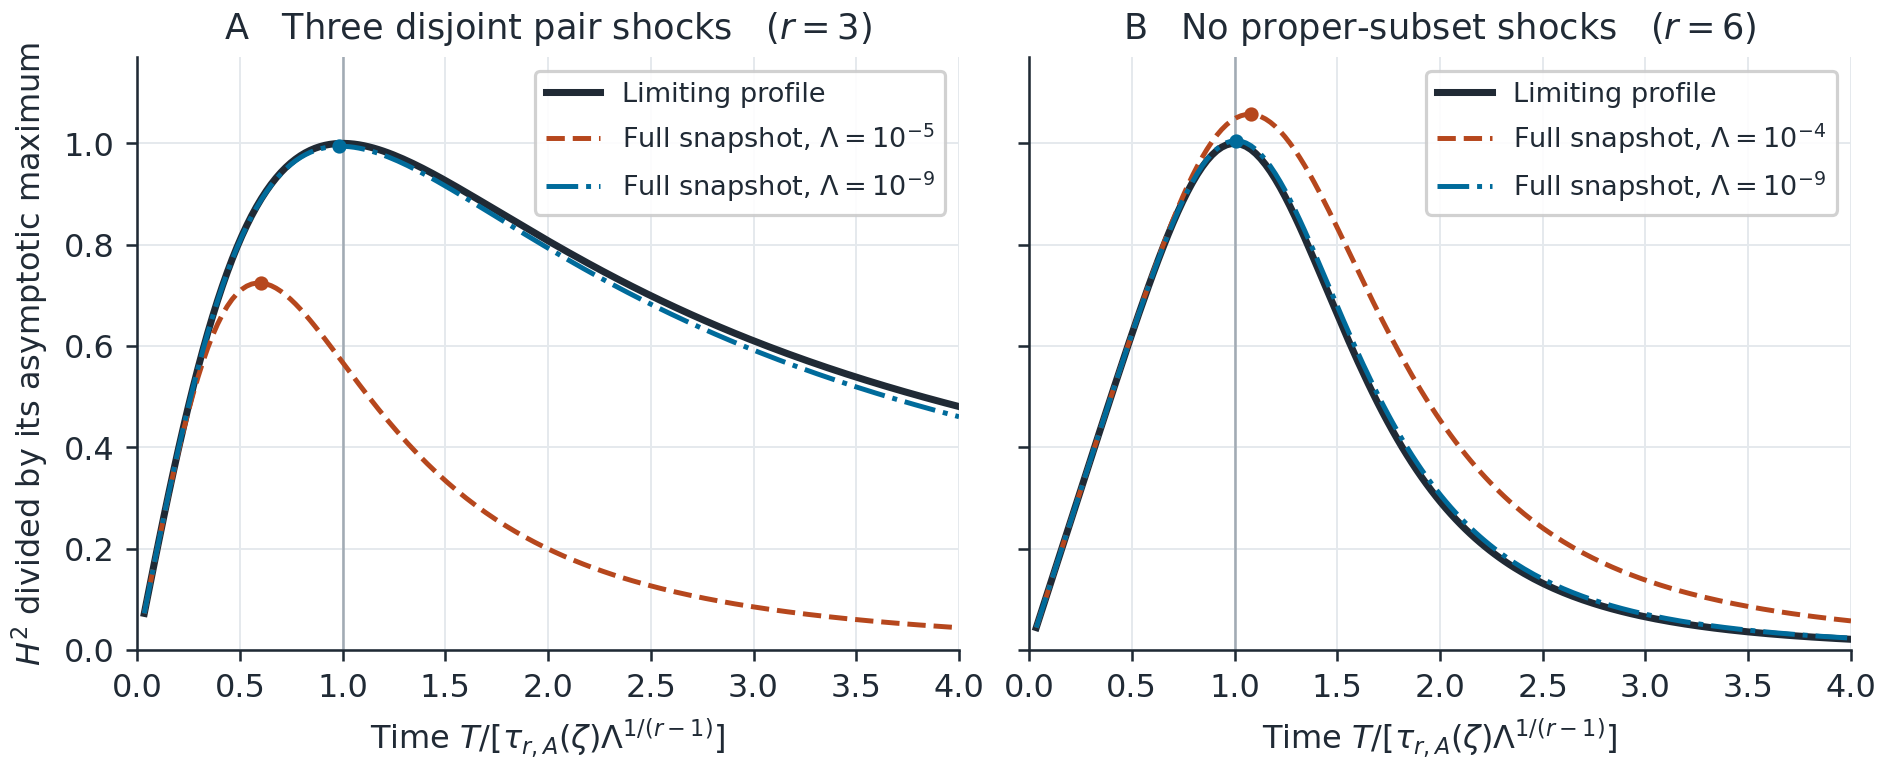
\includegraphics[width=\linewidth]{fixed-dimension-profile.png}
\caption{Fixed-dimensional profiles and numerically evaluated full-snapshot distances for three disjoint pair shocks of rate \(1/5\) each (\(r=3,\ A=1/125\)) and for no background shocks (\(r=6,\ A=64\)). Both use six blocks, \(a=k=1\) and \(\zeta=0.6\). Times and distances are divided by the predicted maximizing time and height. The dots mark grid maxima.}
\label{fig:figure1}
\end{figure}

\begin{figure}[!htbp]
\centering
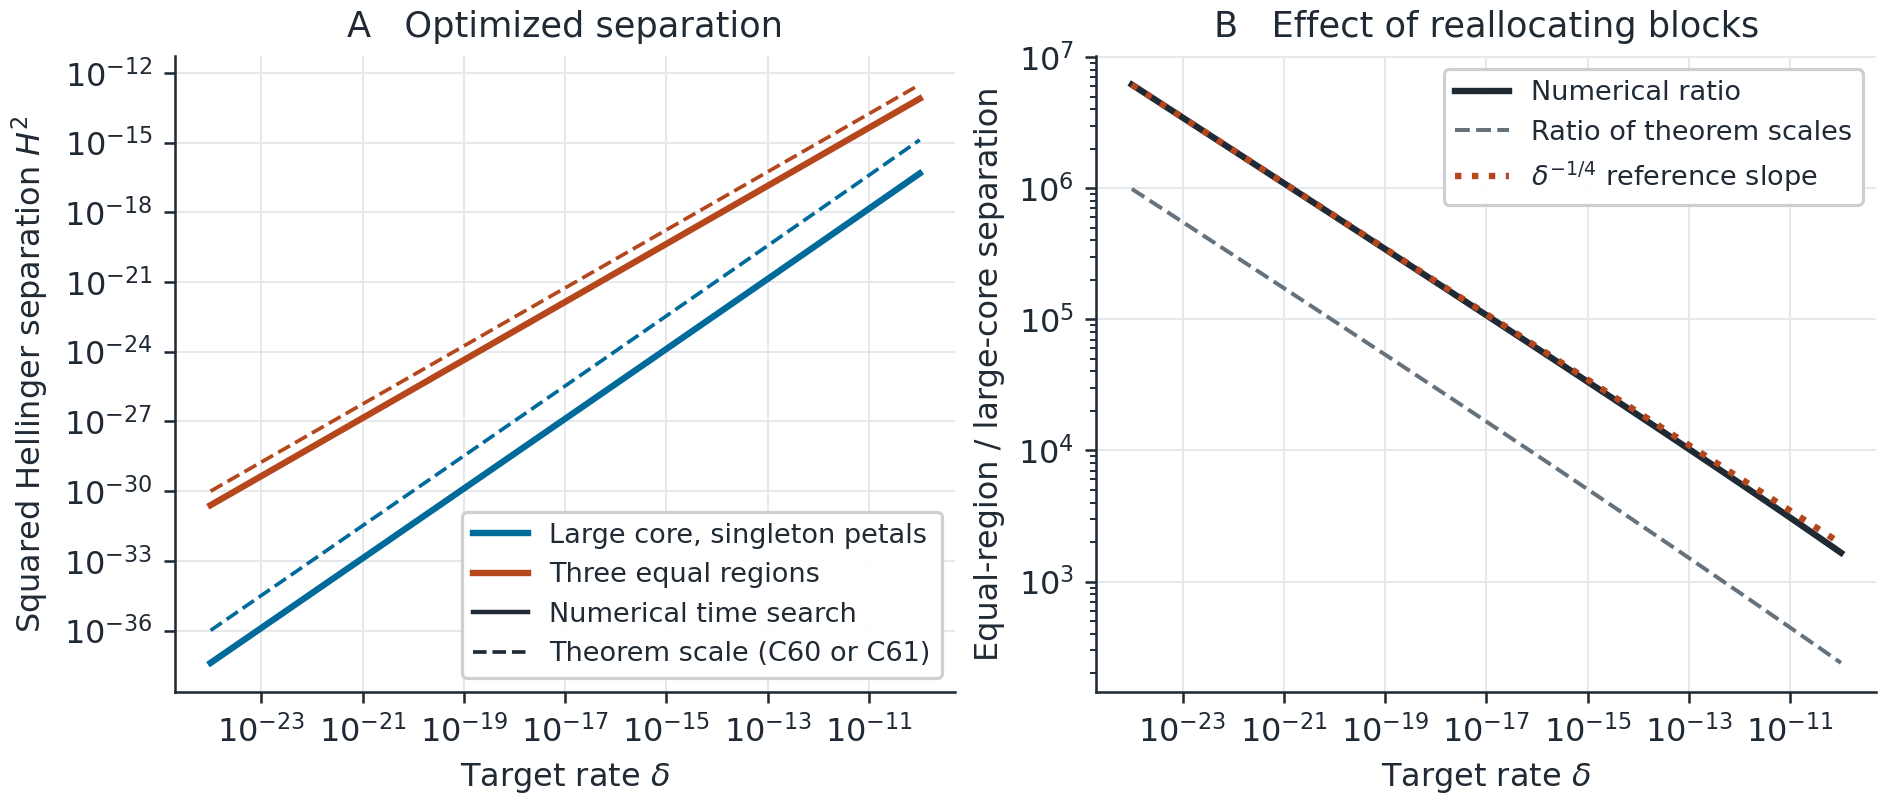
\includegraphics[width=\linewidth]{growing-overlap-comparison.png}
\caption{Two geometries with matched global and background rates and marginal calibration. Both use \(s=3\lceil\delta^{-1/2}/3\rceil\), \(a=k=1\), \(\lambda_0=0,\lambda_1=\delta\), and \(\beta_i=\delta^{3/8}\). The theoretical slopes are \(3/2\) for the large core and \(5/4\) for the large petals. The solid lines in panel A are lower bounds on the unrestricted time supremum obtained from a locally refined time grid. Dashed lines use the comparison scales in (14)--(15). Panel B takes the ratio of the searched values as a numerical illustration.}
\label{fig:figure2}
\end{figure}

For the first figure we sum the full-state square-root distances directly. For the second figure we group full snapshots by the set of regions that are completely covered, then evaluate affinity by summing the product terms for the remaining region patterns.

\clearpage
\section{Discussion}\label{discussion}

At fixed dimension with \(r\ge3\), the order of the leading reliability term determines the scale on which an accidental completion and a global shock contribute comparable mass to the complete cell. Equation (8) explains why optimizing this cell alone gives the first-order optimum in that regime. At order two, finite-time differences in the remaining cells can affect the leading coefficient. The full Fisher curve then determines the optimal design.

For two overlapping backgrounds in growing dimension, a large common core can be completed by either background, leaving at most one easily completed singleton petal. With two large petals, each can remain difficult to complete unless its own background acts. This accounts for the separately saturated probabilities in (15). The two-geometry comparison requires given supports and a shared nonempty core. Questions beyond the present parameter ranges include unknown background rates, vanishing leading coefficients, additional growth regimes, and observation cost that depends on exposure time.

\begingroup
\linespread{0.96}\small
\begin{thebibliography}{99}
\setlength{\itemsep}{0pt}
\setlength{\parsep}{0pt}
\bibitem{aickin2010} Aickin, M. (2010). The Linkset Model for \(2^n\) Contingency Tables. \emph{COBRA Preprint Series}, Paper 68. \href{https://citeseerx.ist.psu.edu/document?doi=28f930b5906fcd41df3e501ad4ecb4f0842f99b7&repid=rep1&type=pdf}{Author manuscript}.

\bibitem{baghel2024} Baghel, S. and Mondal, S. (2024). Robust estimation of dependent competing risk model under interval monitoring and determining optimal inspection intervals. \emph{Applied Stochastic Models in Business and Industry}, 40(4), 926--944. \href{https://doi.org/10.1002/asmb.2854}{DOI}.

\bibitem{boyles1983} Boyles, R. A. and Samaniego, F. J. (1983). Maximum Likelihood Estimation for a Discrete Multivariate Shock Model. \emph{Journal of the American Statistical Association}, 78, 445--448. \href{https://doi.org/10.1080/01621459.1983.10477992}{DOI}.

\bibitem{boyles1984} Boyles, R. A. and Samaniego, F. J. (1984). Modeling and Inference for Multivariate Binary Data with Positive Dependence. \emph{Journal of the American Statistical Association}, 79, 188--193. \href{https://doi.org/10.1080/01621459.1984.10477083}{DOI}.

\bibitem{deldossi2019} Deldossi, L., Osmetti, S. A. and Tommasi, C. (2019). Optimal design to discriminate between rival copula models for a bivariate binary response. \emph{TEST}, 28, 147--165. \href{https://doi.org/10.1007/s11749-018-0595-1}{DOI}.

\bibitem{ding2004} Ding, A. A. and Wang, W. (2004). Testing Independence for Bivariate Current Status Data. \emph{Journal of the American Statistical Association}, 99(465), 145--155. \href{https://doi.org/10.1198/016214504000000142}{DOI}.

\bibitem{esary1967} Esary, J. D., Proschan, F. and Walkup, D. W. (1967). Association of Random Variables, with Applications. \emph{The Annals of Mathematical Statistics}, 38(5), 1466--1474. \href{https://doi.org/10.1214/aoms/1177698701}{DOI}.

\bibitem{jewell2005} Jewell, N. P., van der Laan, M. and Lei, X. (2005). Bivariate current status data with univariate monitoring times. \emph{Biometrika}, 92(4), 847--862. \href{https://doi.org/10.1093/biomet/92.4.847}{DOI}.

\bibitem{kvam1996} Kvam, P. H. (1996). Maximum Likelihood Estimation and the Multivariate Bernoulli Distribution. In \emph{Lifetime Data: Models in Reliability and Survival Analysis}, pp.~187--194. \href{https://doi.org/10.1007/978-1-4757-5654-8_25}{DOI}.

\bibitem{lin2019} Lin, Y., Martin, R. and Yang, M. (2019). On Optimal Designs for Nonregular Models. \emph{The Annals of Statistics}, 47(6), 3335--3359. \href{https://doi.org/10.1214/18-AOS1780}{DOI}.

\bibitem{liu2007} Liu, H.-K. (2007). D- and Ds-optimal Designs for Estimation of Parameters in Bivariate Copula Models. Master's thesis, National Sun Yat-sen University. \href{https://ethesys.lis.nsysu.edu.tw/ETD-db/ETD-search-c/view_etd?URN=etd-0727107-163046}{University repository}.

\bibitem{marichal2016} Marichal, J.-L. (2016). Structure Functions and Minimal Path Sets. \emph{IEEE Transactions on Reliability}, 65, 763--768. \href{https://doi.org/10.1109/TR.2015.2513017}{DOI}.

\bibitem{marshall1967} Marshall, A. W. and Olkin, I. (1967). A Multivariate Exponential Distribution. \emph{Journal of the American Statistical Association}, 62, 30--44. \href{https://doi.org/10.1080/01621459.1967.10482885}{DOI}.

\bibitem{nagaraja2015} Nagaraja, H. N. and He, Q. (2015). Fisher Information in Censored Samples from the Marshall--Olkin Bivariate Exponential Distribution. \emph{Communications in Statistics--Theory and Methods}, 44(19), 4172--4184. \href{https://doi.org/10.1080/03610926.2014.972565}{DOI}.

\bibitem{pensia2024} Pensia, A., Jog, V. and Loh, P.-L. (2024). The Sample Complexity of Simple Binary Hypothesis Testing. \emph{Proceedings of the 37th Conference on Learning Theory}, PMLR 247, 4205--4206. \href{https://proceedings.mlr.press/v247/pensia24a.html}{Proceedings}.
\end{thebibliography}
\endgroup
\end{document}
